\chapter{Technologie}

\section{System oznaczania zębów}
\subsection{Klient}

Vue.js, który został wykorzystany do realizacji modułu diagramu zębowego, to progresywny framework JavaScript umożliwiający implementację interfejsu użytkownika. Technologia ta powstała w~2014 roku i~cały czas się rozwija. Jej podstawowa biblioteka skupia się na tworzeniu warstwy widoku aplikacji i~w połączeniu z~bibliotekami pomocniczymi nadaje się do implementacji zaawansowanych aplikacji jednostronicowych. Aplikacje takie, właściwie nazywane Single-Page Application (SPA), charakteryzują się inną niż domyślna metodą ładowania stron. Rozwiązanie to pozwala na dynamiczną aktualizację jedynie poszczególnych komponentów aplikacji, unikając odświeżenia całej strony dla każdej, nawet małej zmiany.

\begin{figure}[ht!]
\centering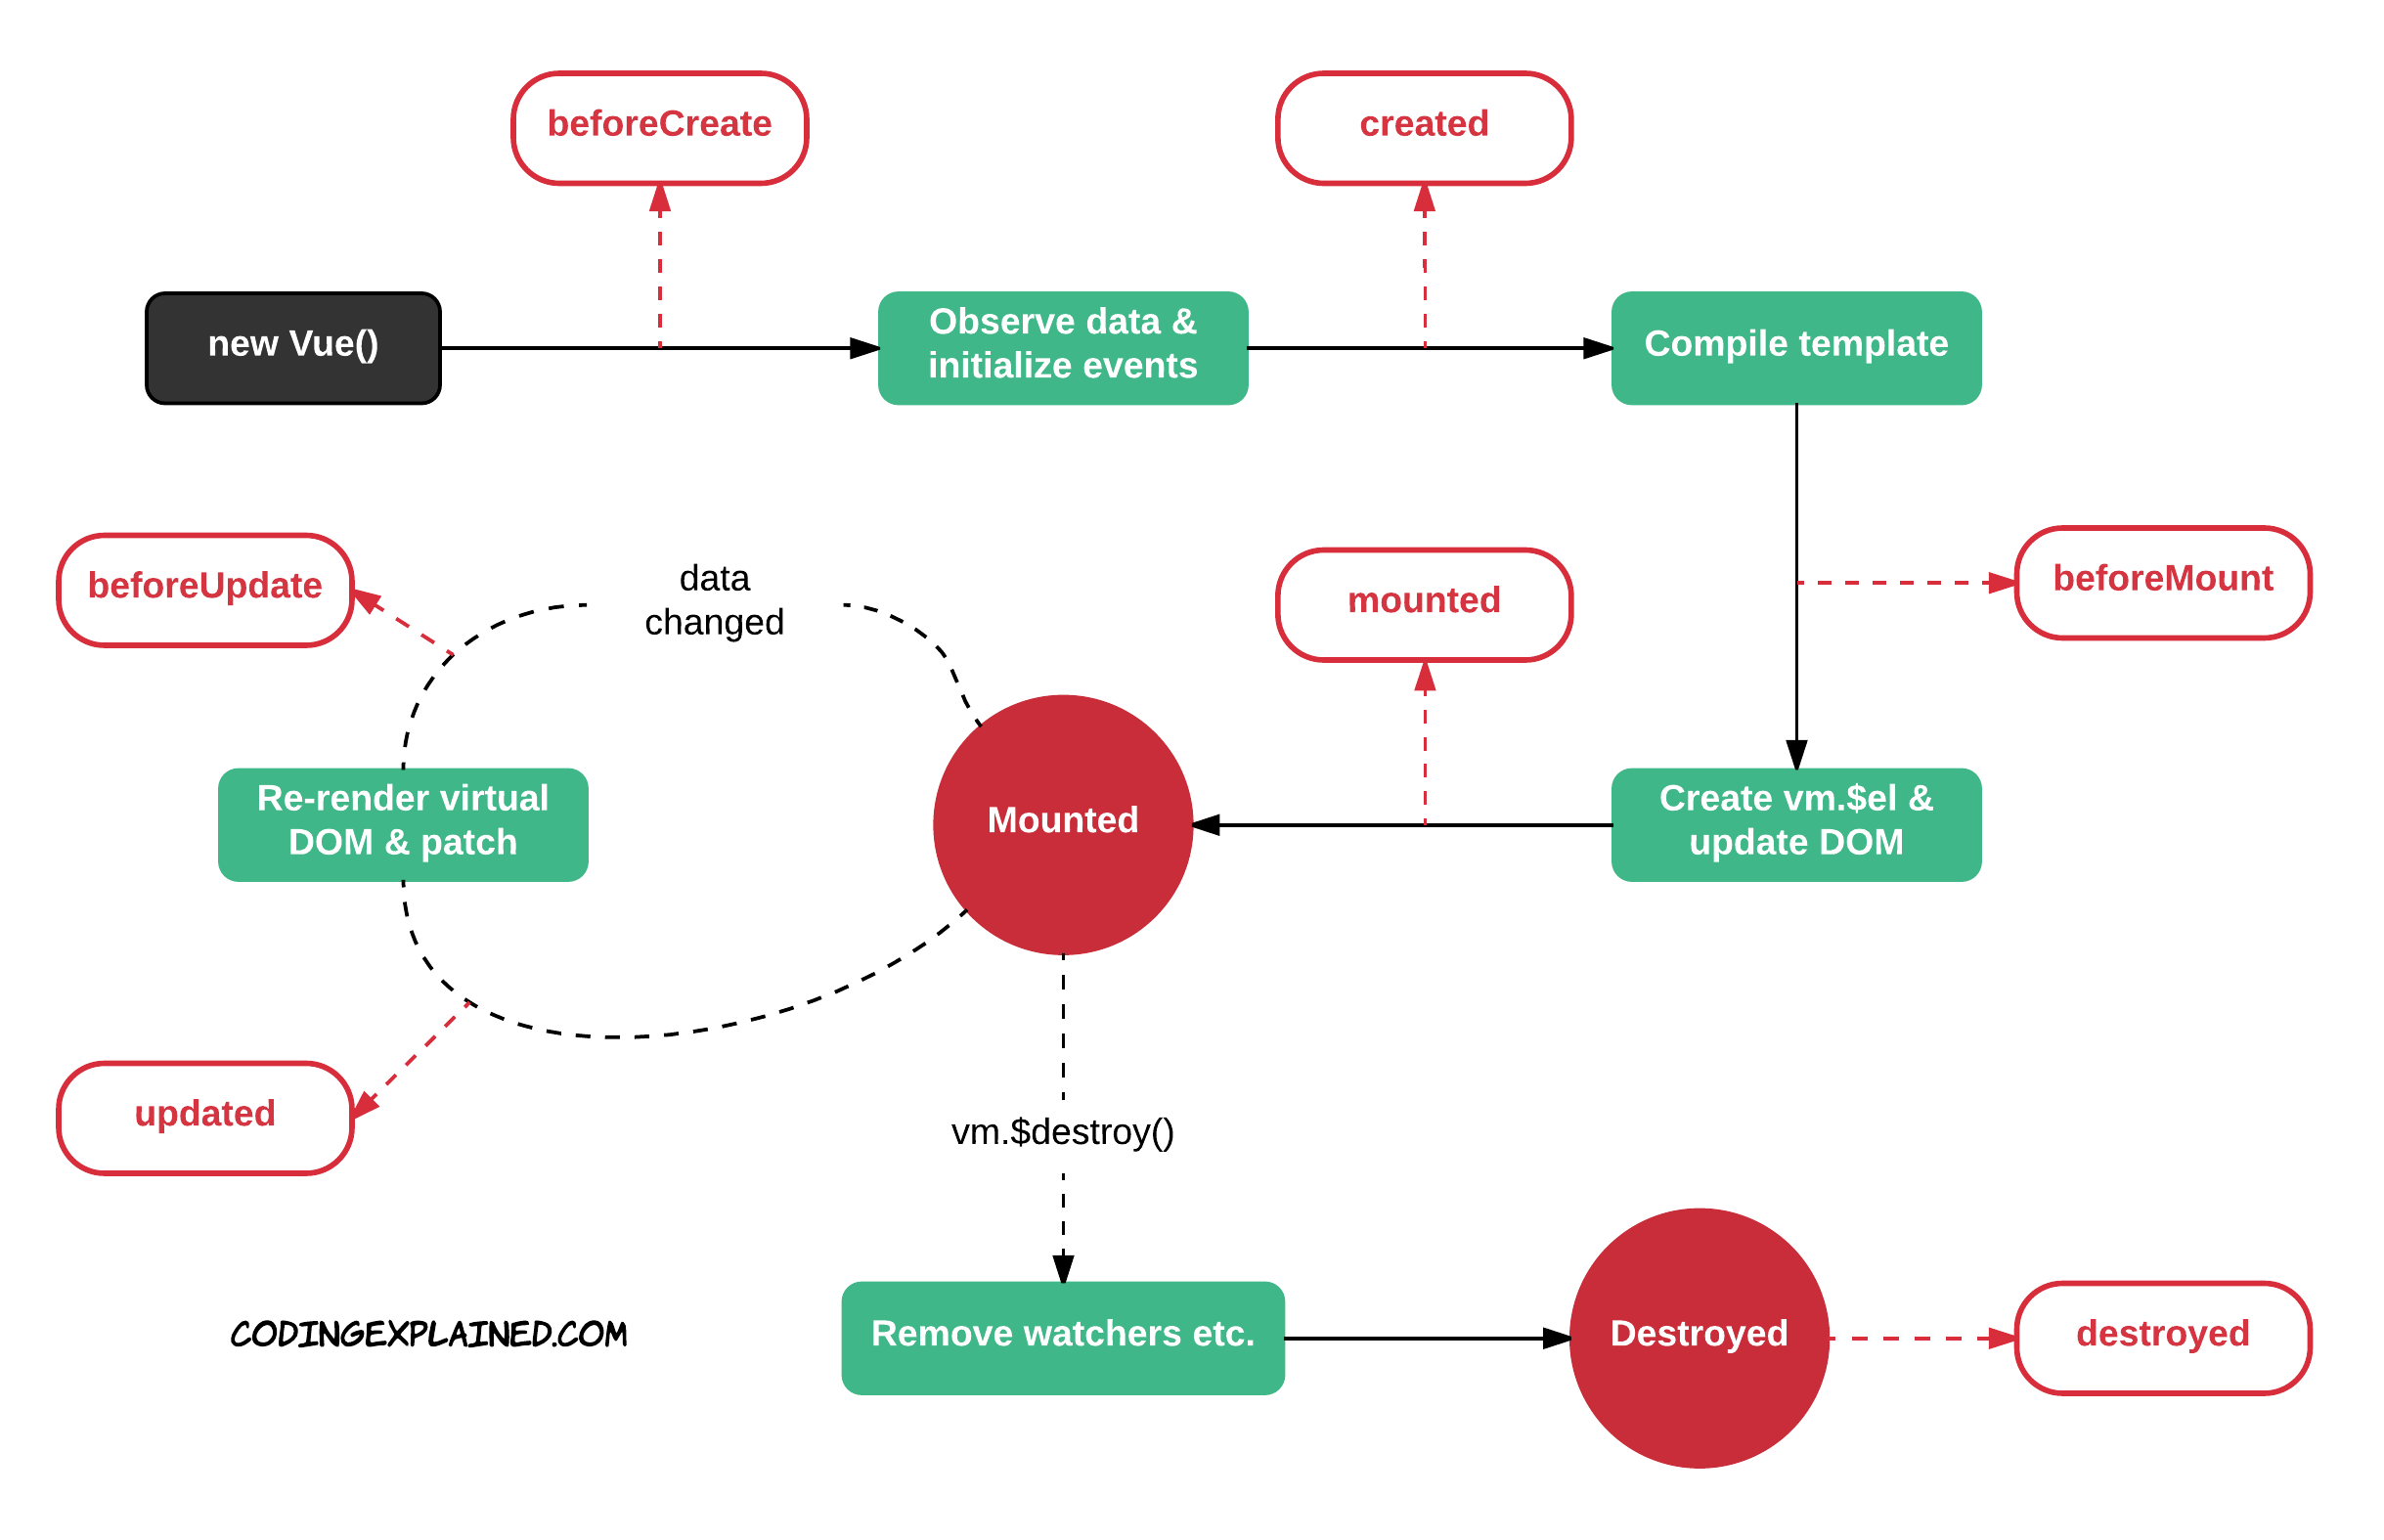
\includegraphics[width=\textwidth]{figures/Vue-instance-lifecycle-Page-1.png}
\caption{Diagram przedstawiający cykl życia instancji Vue\cite{vueLifeCycle}}
\label{fig:vuepopularity}
\end{figure}

Utworzenie aplikacji Vue jest jednoznaczne z~utworzeniem nowej instancji Vue (najczęściej oznaczanej jako vm), która składa się z~odrębnych komponentów. Działanie takiej aplikacji, a~właściwie poszczególnych jej komponentów, można w~prosty sposób przedstawić na diagramie, który nazywany jest cyklem życia Vue. Dla każdego komponentu aplikacji definiuje się zbiór właściwości oraz metod, które są wykorzystywane podczas działania programu. Pewien ściśle określony zbiór zmiennych jest reaktywny, co oznacza, że program wykrywa ich zmiany i~w razie ich edycji aktualizuje komponent używając nowo zdefiniowanych wartości i~ponownie go renderując.\cite{vuejs}

\begin{itemize}
\item koniecznie pros and cons - https://www.altexsoft.com/blog/engineering/pros-and-cons-of-vue-js/
\item w~kwestii diagramu działania Vue ,można opisać DOM - https://blog.logrocket.com/how-the-virtual-dom-works-in-vue-js/
\end{itemize}

\subsection{Serwer}
Serwer jest miejscem komunikacji wszystkich komponentów aplikacji. Jest odpowiedzialny za przetwarzanie żądań klienta oraz za łączność z~bazą danych i~z API do rozpoznawania mowy. Do implementacji serwera użyty został język Python oraz micro-framework Flask. 

\subsubsection{Flask}
Flask nazywany jest webowym mikro-frameworkiem. Przedrostek ,,mikro`` oznacza, że posiada prosty i~zajmujący mało miejsca pamięci rdzeń \cite{flaskdoc}. Jednakże jest zbudowany tak aby był modułowy i~bardzo elastyczny dla deweloperów. Flask nie posiada domyślnie takich funkcjonalności jak: ORM, arkusze walidacyjne, obsługa przekazywania plików czy systemów uwierzytelniania. Jak wspomniano wcześniej, framework posiada cechy, które pozwalają na proste użycie rozszerzeń. Dzięki czemu można uzupełnić funkcjonalności, w~sposób dopasowany do aktualnego projektu.
Flask jest frameworkiem WSGI. Oznacza to, że jest zgodny ze standardem języka Python o~nazwie PEP-3333. Standard zapewnia prostotę i~kompatybilność komunikacji między serwerem a~klientem dla aplikacji webowych w~języku Python\cite{pep3333}.

Budowa frameworka Flask bazuje na dwóch komponentach\cite{flaskdoc}:
\begin{itemize}
\item Jinja2 - silnik szablonów 
\item Werkzeug - biblioteka narzędzi do obsługi WSGI
\end{itemize}

Głównym zadaniem, do którego użyto powyższego frameworka jest obsługa żądań poprzez zaimplementowane węzły końcowe. Serwer jest uruchomiony w~tle i~działając nieprzerwanie, oczekuje na żądania. Serwer obsługuje zapytania POST w~komunikacji z~frontendem oraz bazą danych. Odpowiada również za rejestracje komend głosowych, połączenie z~API do rozpoznawania mowy oraz weryfikacji poprawności komend.

\subsubsection{MongoDB}
Technologią użytą do magazynowania oraz przetwarzania danych jest MongoDB. Jest to nierelacyjny system zarządzania bazami danych. Bazy MongoDB są przeznaczone do projektów gdzie istotna jest skalowalność oraz łatwy rozwój\cite{mongoDoc}. MongoDB jest zorientowane na dokumenty. Oznacza to, że zamiast tabel i~wierszy, jak w~relacyjnych bazach danych, używa kolekcji oraz dokumentów. Dokument jest tworzony w~stylu JSON, zawiera więc pary kluczy-wartości. Takie pary są podstawową jednostką danych w~technologi MongoDB. Kolekcje są zbiorem dokumentów.

Bazy danych MongoDB z~uwagi na typ NoSQL, posiadają pewne zalety:\cite{noSql}. 
\begin{itemize}
\item Duża skalowalność 
\item Elastyczny model obiektów danych
\item Przechowywanie masywnych danych
\item Prosta obsługa i~tanie utrzymanie
\item Szeroka konkurencja - duży wybór 
\item Duża liczba rozwiązań open-source
\end{itemize}
Bazy nierelacyjne nie są jednak najlepszym rozwiązanie do każdego projektu. Posiadają pewne wady w~stosunku do baz relacyjnych:\cite{noSql}. 
\begin{itemize}
\item Często z~uwagi na charakter open-source, nie posiadają pełnego wsparcia użytkownika
\item Nie posiadają wspólnego języka zapytań
\item Ewentualne błędy w~danych są trudne do wykrycia, z~uwagi na elastyczne modele danych
\end{itemize}

\begin{figure}[ht!]
\centering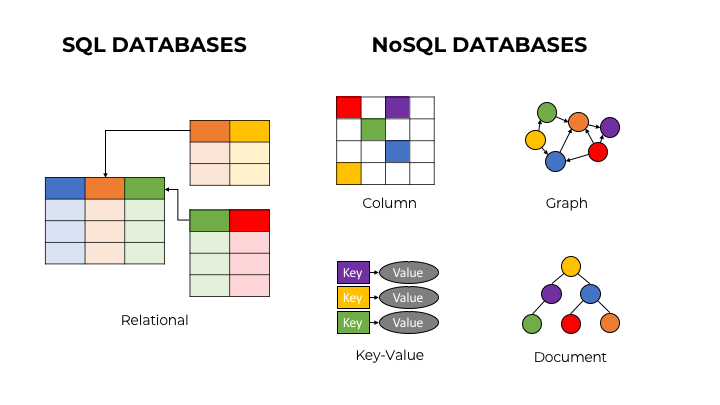
\includegraphics[width=\textwidth]{figures/sqlvsnosql.png}
\caption{Różnice między strukturami danych w~bazach danych typu relacyjnego (SQL) oraz bazach danych typu nierelacyjnego (NoSQL).}
\label{fig:sqlvsnosql}
\end{figure}

Wybór technologi MongoDB do realizacji projektu, był podyktowany prostotą wprowadzania zmian w~strukturze danych. W~szczególności możliwością rozszerzania aplikacji o~inne moduły, których model danych jest inny od obecnego w~aplikacji.
\subsection{Zewnętrzne API}
\subsubsection{Rozpoznawanie mowy}
Interfejs głosowy poprzez, który użytkownik może wprowadzać dane komendami głosowymi w~języku polskim, wymaga zaawansowanego rozwiązania. W~tym celu użyta została biblioteka Speech-Recognition w~języku Python\cite{pythonSpeech}. Główną funkcjonalnością biblioteki jest przetworzenie mowy na tekst. Wykorzystuje do tego kilka gotowych API dostępnych w~internecie. Do projektu zostało wybrane Google Speech Recognition API, które wykorzystuje Web Speech API\cite{webSpeechApi}.

Biblioteka \textbf{Python Speech Recognition} pozwala w~prosty sposób użyć swojej funkcjonalności w~projekcie. Cały proces zmieniający mowę na tekst, zawiera następujące kroki:
\begin{itemize}
\item Pobranie danych dźwiękowych z~mikrofonu bądź pliku
\item Przetworzenie danych dźwiękowych
\item Przesłanie żądania z~przetworzonymi danymi do Google Speech Recognition API
\item Odebranie odpowiedzi w~formie łańcucha tekstu
\end{itemize}

Wymogiem łączności z~API do rozpoznawania mowy jest łączność z~internetem. API jest dostępne publicznie do celów niekomercyjnych i~testowych\cite{webSpeechApi}. W~przypadku wydania aplikacji projektowej lub skomercjalizowania jej, jest możliwość zmiany API na Google Cloud API. Wiąże się to z~opłatami, jeżeli API przetwarza więcej niż 60 minut miesięcznie\cite{cloudSpeechAPI}. Każde żądanie jest rozumiane jako minimum 15 sekund. Można przyjąć, że w~aplikacji jedna komenda głosowa to jedno żądanie do API. Miesięcznie darmowe jest więc 240 komend głosowych. Za każde dodatkowe żądanie do 15 sekund należy zapłacić 0.006 dolara amerykańskiego. Przy kursie walutowym na poziomie 3,69 PLN za 1 USD, jedna komenda kosztuje 0,022 PLN.

W przypadku stomatologa, który realizuje 10 wizyt dziennie i~przy każdej z~nich wypowiada 6 komend głosowych oraz pracuje 22 dni robocze w~miesiącu. Lekarz wypowie 1320 komend miesięcznie, od czego należy odjąć 240 komend darmowych - co równa się 1080 żądań za kwotę 23,76 PLN. Dla tych samych założeń ale 10 komend poprawnych i~2 komend błędnych na wizytę, kwota miesięczna to 52,88 PLN.

\begin{figure}[ht!]
\centering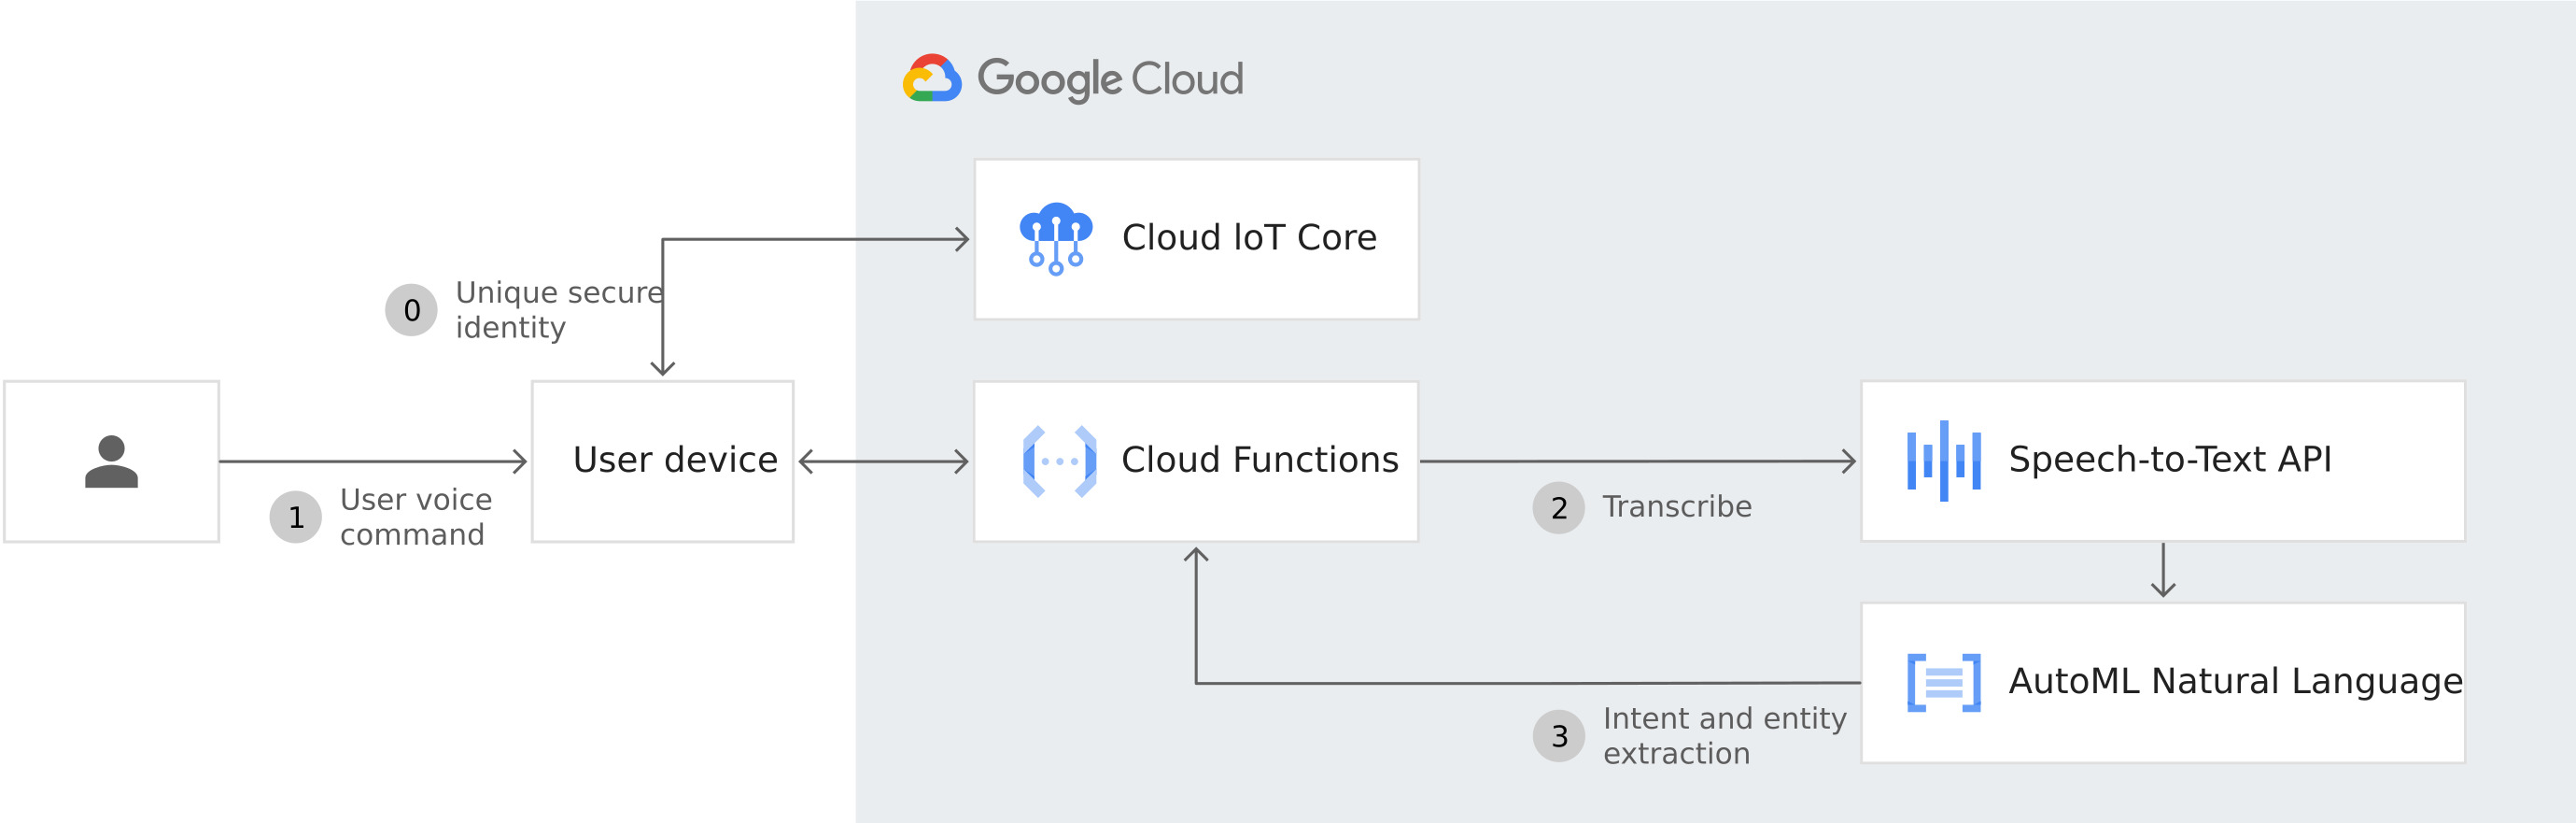
\includegraphics[width=\textwidth]{figures/googleCloudDiagram.jpg}
\caption{Diagram sposobu działania Google Cloud Speech Recognition API.\cite{cloudSpeechAPI}}
\label{fig:googleCloudDiagram}
\end{figure}



\section{Analiza odchylenia toru odwodzenia żuchwy}

\subsection{Wykorzystane biblioteki}

\subsubsection{Biblioteka NumPy}
NumPy (Numerical Python) to biblioteka open-source dostarczająca narzędzi do prowadzenia obliczeń na macierzach i tablicach wielowymiarowych \cite{numpy}. Z powodu wysokiej wydajności i prostoty przetwarzania na oferowanych przez siebie strukturach danych, NumPy stanowi dziś standard w niemal każdym naukowym i technicznym zastosowaniu języka Python. Tablice NumPy to w matematycznym sensie tensory, dlatego biblioteka umożliwia łatwą implementację modeli teoretycznych wyrażonych za pomocą algebry liniowej. Z uwagi na naturalną reprezentację, struktury danych oferowane przez bibliotekę w praktyce stanowią najpopularniejszy format transferu danych w naukowo-technicznym ekosystemie języka Python, czego dowodem może być łańcuch zależności przedstawiony na diagramie \ref{fig:numpy_applications}.

\begin{figure}
\centering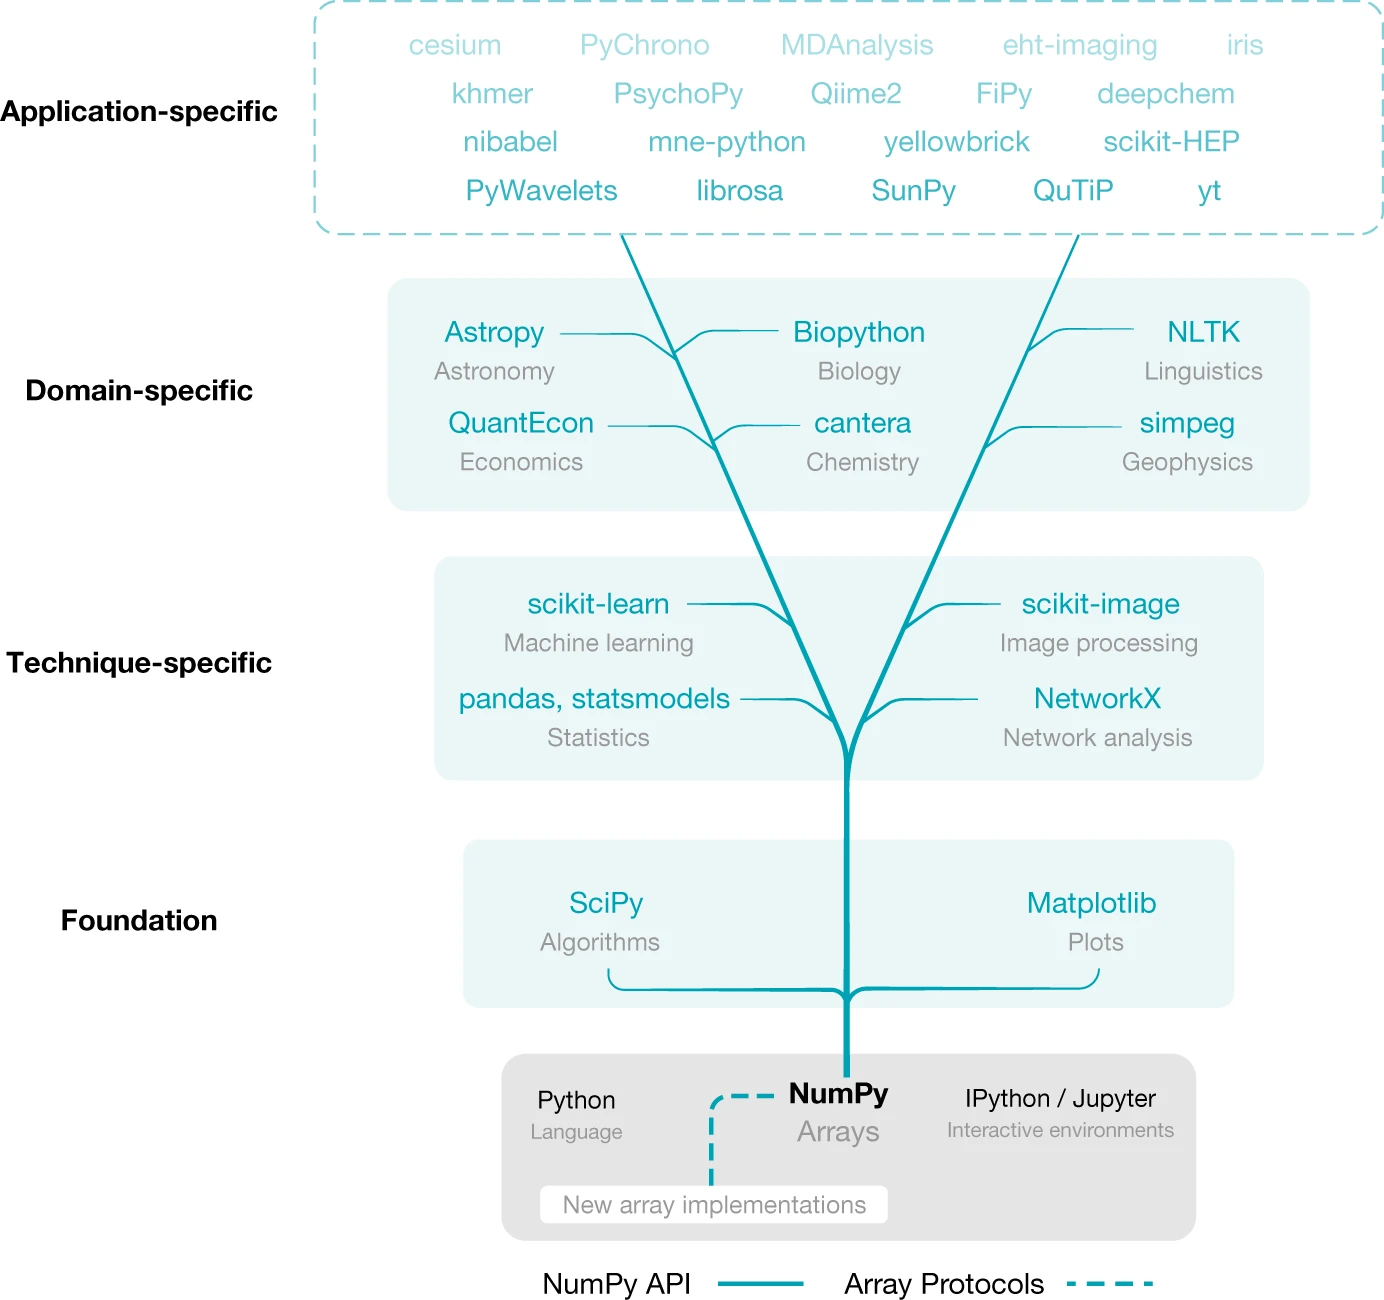
\includegraphics[width=100mm]{figures/numpy.png}
\caption{Miejsce biblioteki NumPy wśród narzędzi języka Python \cite{numpy}}
\label{fig:numpy_applications}
\end{figure}


\subsubsection{Biblioteka OpenCV}
Open Source Computer Vision Library\cite{opencv} to biblioteka funkcji zajmująca się przetwarzaniem obrazu oraz uczeniem maszynowym. Została zaprojektowana, aby dostarczyć łatwo dostępną infrastrukturę do tworzenia przetwarzających obraz aplikacji w~czasie rzeczywistym. Miała również przyspieszyć użycie podejścia maszynowego w~komercyjnych produktach. Dzięki oparciu na otwartym kodzie, pozwala firmą eksploatować i~rozwijać kod. Biblioteka OpenCV zawiera około 2500 zoptymalizowanych algorytmów, które oprócz klasycznych podejść do przetwarzania obrazów i~uczenia maszynowego, wyczerpują temat również w~zakresie najnowocześniejszych pomysłów. Algorytmy mogą zostać wykorzystane do np.:
\begin{itemize}
    \item Wykrycia i~rozpoznania ludzkiej twarzy
    \item Identyfikowania obiektów
    \item Przyporządkowywania ludzkich zachowań w~filmach
    \item Śledzenia poruszających się elementów w~filmach
    \item Uzyskania modelów 3D z~obiektów
    \item Składania obrazów w~jeden, aby pokazać obraz całej przestrzeni w~wysokiej rozdzielczości
    \item Znajdowania podobnego obrazu w~bazie danych
    \item Śledzenie ruchu gałek ocznych
    \item Usuwanie czerwonych gałek ocznych ze zdjęć
\end{itemize}
Biblioteka znajduje szerokie zastosowanie w~firmach i~grupach badawczych.
W projekcie zostały użyte różne funkcje z~biblioteki dotyczące śledzenia obiektów, wyświetlania i~obsługi filmów, transformację obrazu z~różnych przestrzeni barw.

\subsubsection{Biblioteka scikit-image}
scikit-image (skimage) to kolejna poświęcona przetwarzaniu obrazów biblioteka języka Python. Dostarcza ona algorytmów oraz narzędzi poświęconych badaniom, edukacji i zastosowaniom komercyjnym. Jej twórcy podkreślają prostotę interfejsu programistycznego i jakość dokumentacji, znacznie ułatwiające naukę zarówno w formie samodzielnej eksploracji, jak i zorganizowanych kursów. Biblioteka scikit-image rozpowszechniana jest w ramach bardzo liberalnej licencji \emph{Modified BSD}, zapewniającej pełną możliwość modyfikacji kodu, ale również wykorzystywania w zamkniętym oprogramowaniu. W obliczu faktu znacznego pokrywania się funkcjonalności scikit-image z OpenCV, warto podkreślić różnice pomiędzy tymi bibliotekami. Logika OpenCV zaimplementowana jest w językach C i C++, co powoduje bardziej proceduralny, niskopoziomowy sposób obsługi jej interfejsu dla języka Python. Z kolei scikit-image jest w pełni dopasowana do filozofii i stylu technologii Python, umożliwiając programowanie zgodne z podejściem imperatywnym lub funkcyjnym. Ponadto dostarcza ona nie tylko algorytmów z dziedziny widzenia komputerowego, lecz także przetwarzania obrazów medycznych i mikroskopowych \cite{skimage}.

\subsubsection{Biblioteka Tkinter}
Biblioteka Tkinter\cite{tkinter} to standardowe narzędzie w~języku Python, używane do tworzenia graficznego interfejsu użytkownika. Jest dostępny na większości platform Unix, a~także na systemach Windows.
Został wykorzystany, aby stomatolog mógł łatwo wybrać i~przetworzyć przechowywane na komputerze filmy.

\subsection{Interfejs programistyczny przetwarzania obrazów}

Zdjęcia i nagrania uzyskane metodami fotografii cyfrowej tworzone są w procesie naświetlania matrycy, tworzącej dyskretną reprezentację wizualną sceny. Z tego powodu wszystkie niskopoziomowe techniki przetwarzania obrazu zakładają implementację grafiki w formie rastrowej. Oznacza to, że dane przechowywane są w formie tablicy wielowymiarowej, w której najmniejszą jednostką jest piksel. Informacja o względnym położeniu punktów obrazu odwzorowana jest w indeksy poszczególnych pikseli, natomiast intensywność punktów kodowana jest w formie skalara (w przypadku obrazów monochromatycznych) lub wektora o trzech składowych (w reprezentacjach wielokolorowych).  

Współczesne kamery są w stanie zbierać ilości informacji znacznie przekraczające czułość ludzkiej percepcji. Co więcej obrazy przedstawiające rzeczywiste obiekty cechują się znaczną regularnością, w stosunku do wszystkich możliwych macierzy o danym kształcie \cite{image_svd}. Z tych względów wynaleziono bardzo wiele metod kompresji obrazów, i co za tym idzie, formatów plików do ich przechowywania. Standardowe narzędzia programistyczne (jak scikit-image czy OpenCV) zapewniają abstrakcję reprezentacji wczytywanego pliku i zwracają zdekompresowaną informację w formie tablicy liczb zmiennoprzecinkowych w ustalonej przestrzeni barw \cite{learning_opencv}.

Z racji tego, że filmy to zwyczajnie sekwencje obrazów o ustalonych odstępach czasowych, interfejs analizy nagrań definiowany jest zarówno w scikit-image, jak i w OpenCV, w formie strumienia klatek. Strumieniowy sposób przetwarzania pozwala pominąć kwestie długości nagrania czy liczby klatek na sekundę i przetwarzać kolejne próbki w identyczny sposób jak samodzielne obrazy. Oczywiście pożądane może być przechowywanie informacji o zmianach danych w czasie, ale realizuje się je poza interfejsem wczytywania nagrania.

\begin{figure}
    \centering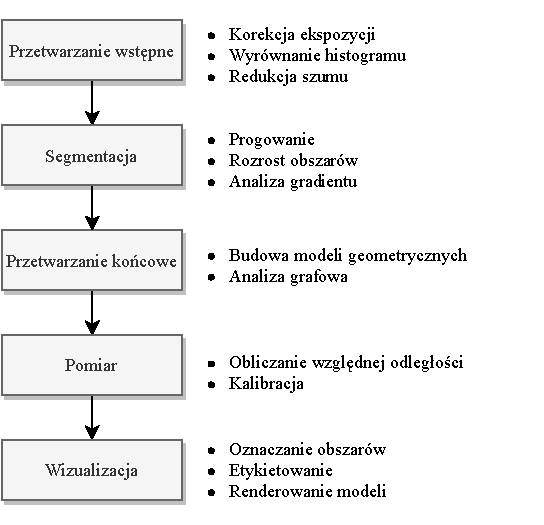
\includegraphics[width=100mm]{figures/Diagram przetwarzania.pdf}
    \caption{Diagram etapów przykładowego procesu przetwarzania obrazów}
    \label{fig:image_pipeline}
\end{figure}

Struktury danych będące wynikiem algorytmów wyższego poziomu niż wejściowe obrazy w większym stopniu zależą od decyzji twórców danej biblioteki. Często wykorzystywane są typowe kształty geometryczne, jednak ich implementacje w różnych bibliotekach mogą nie być ze sobą kompatybilne. Konieczne jest wówczas zachowanie ostrożności przy równoczesnym wykorzystaniu funkcji o różnych reprezentacjach obiektów mających tę samą interpretację (jak na przykład w przypadku prostokąta w bibliotekach scikit-image oraz OpenCV).

